% Options for packages loaded elsewhere
\PassOptionsToPackage{unicode}{hyperref}
\PassOptionsToPackage{hyphens}{url}
\documentclass[
]{article}
\usepackage{xcolor}
\usepackage[margin=1in]{geometry}
\usepackage{amsmath,amssymb}
\setcounter{secnumdepth}{-\maxdimen} % remove section numbering
\usepackage{iftex}
\ifPDFTeX
  \usepackage[T1]{fontenc}
  \usepackage[utf8]{inputenc}
  \usepackage{textcomp} % provide euro and other symbols
\else % if luatex or xetex
  \usepackage{unicode-math} % this also loads fontspec
  \defaultfontfeatures{Scale=MatchLowercase}
  \defaultfontfeatures[\rmfamily]{Ligatures=TeX,Scale=1}
\fi
\usepackage{lmodern}
\ifPDFTeX\else
  % xetex/luatex font selection
\fi
% Use upquote if available, for straight quotes in verbatim environments
\IfFileExists{upquote.sty}{\usepackage{upquote}}{}
\IfFileExists{microtype.sty}{% use microtype if available
  \usepackage[]{microtype}
  \UseMicrotypeSet[protrusion]{basicmath} % disable protrusion for tt fonts
}{}
\makeatletter
\@ifundefined{KOMAClassName}{% if non-KOMA class
  \IfFileExists{parskip.sty}{%
    \usepackage{parskip}
  }{% else
    \setlength{\parindent}{0pt}
    \setlength{\parskip}{6pt plus 2pt minus 1pt}}
}{% if KOMA class
  \KOMAoptions{parskip=half}}
\makeatother
\usepackage{color}
\usepackage{fancyvrb}
\newcommand{\VerbBar}{|}
\newcommand{\VERB}{\Verb[commandchars=\\\{\}]}
\DefineVerbatimEnvironment{Highlighting}{Verbatim}{commandchars=\\\{\}}
% Add ',fontsize=\small' for more characters per line
\usepackage{framed}
\definecolor{shadecolor}{RGB}{248,248,248}
\newenvironment{Shaded}{\begin{snugshade}}{\end{snugshade}}
\newcommand{\AlertTok}[1]{\textcolor[rgb]{0.94,0.16,0.16}{#1}}
\newcommand{\AnnotationTok}[1]{\textcolor[rgb]{0.56,0.35,0.01}{\textbf{\textit{#1}}}}
\newcommand{\AttributeTok}[1]{\textcolor[rgb]{0.13,0.29,0.53}{#1}}
\newcommand{\BaseNTok}[1]{\textcolor[rgb]{0.00,0.00,0.81}{#1}}
\newcommand{\BuiltInTok}[1]{#1}
\newcommand{\CharTok}[1]{\textcolor[rgb]{0.31,0.60,0.02}{#1}}
\newcommand{\CommentTok}[1]{\textcolor[rgb]{0.56,0.35,0.01}{\textit{#1}}}
\newcommand{\CommentVarTok}[1]{\textcolor[rgb]{0.56,0.35,0.01}{\textbf{\textit{#1}}}}
\newcommand{\ConstantTok}[1]{\textcolor[rgb]{0.56,0.35,0.01}{#1}}
\newcommand{\ControlFlowTok}[1]{\textcolor[rgb]{0.13,0.29,0.53}{\textbf{#1}}}
\newcommand{\DataTypeTok}[1]{\textcolor[rgb]{0.13,0.29,0.53}{#1}}
\newcommand{\DecValTok}[1]{\textcolor[rgb]{0.00,0.00,0.81}{#1}}
\newcommand{\DocumentationTok}[1]{\textcolor[rgb]{0.56,0.35,0.01}{\textbf{\textit{#1}}}}
\newcommand{\ErrorTok}[1]{\textcolor[rgb]{0.64,0.00,0.00}{\textbf{#1}}}
\newcommand{\ExtensionTok}[1]{#1}
\newcommand{\FloatTok}[1]{\textcolor[rgb]{0.00,0.00,0.81}{#1}}
\newcommand{\FunctionTok}[1]{\textcolor[rgb]{0.13,0.29,0.53}{\textbf{#1}}}
\newcommand{\ImportTok}[1]{#1}
\newcommand{\InformationTok}[1]{\textcolor[rgb]{0.56,0.35,0.01}{\textbf{\textit{#1}}}}
\newcommand{\KeywordTok}[1]{\textcolor[rgb]{0.13,0.29,0.53}{\textbf{#1}}}
\newcommand{\NormalTok}[1]{#1}
\newcommand{\OperatorTok}[1]{\textcolor[rgb]{0.81,0.36,0.00}{\textbf{#1}}}
\newcommand{\OtherTok}[1]{\textcolor[rgb]{0.56,0.35,0.01}{#1}}
\newcommand{\PreprocessorTok}[1]{\textcolor[rgb]{0.56,0.35,0.01}{\textit{#1}}}
\newcommand{\RegionMarkerTok}[1]{#1}
\newcommand{\SpecialCharTok}[1]{\textcolor[rgb]{0.81,0.36,0.00}{\textbf{#1}}}
\newcommand{\SpecialStringTok}[1]{\textcolor[rgb]{0.31,0.60,0.02}{#1}}
\newcommand{\StringTok}[1]{\textcolor[rgb]{0.31,0.60,0.02}{#1}}
\newcommand{\VariableTok}[1]{\textcolor[rgb]{0.00,0.00,0.00}{#1}}
\newcommand{\VerbatimStringTok}[1]{\textcolor[rgb]{0.31,0.60,0.02}{#1}}
\newcommand{\WarningTok}[1]{\textcolor[rgb]{0.56,0.35,0.01}{\textbf{\textit{#1}}}}
\usepackage{longtable,booktabs,array}
\newcounter{none} % for unnumbered tables
\usepackage{calc} % for calculating minipage widths
% Correct order of tables after \paragraph or \subparagraph
\usepackage{etoolbox}
\makeatletter
\patchcmd\longtable{\par}{\if@noskipsec\mbox{}\fi\par}{}{}
\makeatother
% Allow footnotes in longtable head/foot
\IfFileExists{footnotehyper.sty}{\usepackage{footnotehyper}}{\usepackage{footnote}}
\makesavenoteenv{longtable}
\usepackage{graphicx}
\makeatletter
\newsavebox\pandoc@box
\newcommand*\pandocbounded[1]{% scales image to fit in text height/width
  \sbox\pandoc@box{#1}%
  \Gscale@div\@tempa{\textheight}{\dimexpr\ht\pandoc@box+\dp\pandoc@box\relax}%
  \Gscale@div\@tempb{\linewidth}{\wd\pandoc@box}%
  \ifdim\@tempb\p@<\@tempa\p@\let\@tempa\@tempb\fi% select the smaller of both
  \ifdim\@tempa\p@<\p@\scalebox{\@tempa}{\usebox\pandoc@box}%
  \else\usebox{\pandoc@box}%
  \fi%
}
% Set default figure placement to htbp
\def\fps@figure{htbp}
\makeatother
\setlength{\emergencystretch}{3em} % prevent overfull lines
\providecommand{\tightlist}{%
  \setlength{\itemsep}{0pt}\setlength{\parskip}{0pt}}
\usepackage{bookmark}
\IfFileExists{xurl.sty}{\usepackage{xurl}}{} % add URL line breaks if available
\urlstyle{same}
\hypersetup{
  pdftitle={Unit 4.3: Monte Carlo Integration and Importance Sampling},
  pdfauthor={Dr.~Manoj C. Patil},
  hidelinks,
  pdfcreator={LaTeX via pandoc}}

\title{Unit 4.3: Monte Carlo Integration and Importance Sampling}
\author{Dr.~Manoj C. Patil}
\date{2026-09-30}

\begin{document}
\maketitle

\section{Why Monte Carlo?}\label{why-monte-carlo}

Quadrature (Unit 4.2) puts points on a grid. In \(d\) dimensions the
grid needs (points per axis)\(^d\) evaluations, which quickly becomes
impossible.

Monte Carlo uses \textbf{random points} instead. Its error is about
\(1/\sqrt n\) \textbf{no matter how many dimensions} the integral has.

\section{Monte Carlo Integration}\label{monte-carlo-integration}

\subsection{The idea}\label{the-idea}

An integral is an expectation, and an expectation is estimated by an
average. If \(X \sim f\):

\[
\theta = \int g(x) f(x)\,dx = E[g(X)]
\quad\Longrightarrow\quad
\hat\theta = \frac{1}{n}\sum_{i=1}^n g(X_i)
\]

Two special cases cover most problems:

\begin{itemize}
\tightlist
\item
  \textbf{Integral on \([a,b]\):} \(\int_a^b h(x)\,dx = (b-a)\,E[h(U)]\)
  with \(U \sim \text{Uniform}(a,b)\).
\item
  \textbf{Probability:} \(P(X \in A) = E[\mathbf 1_A(X)]\), which is the
  fraction of draws that land in \(A\).
\end{itemize}

\subsection{Method}\label{method}

\begin{enumerate}
\def\labelenumi{\arabic{enumi}.}
\tightlist
\item
  Draw \(X_1,\dots,X_n\) from \(f\).
\item
  Compute \(g(X_1),\dots,g(X_n)\).
\item
  Estimate \(\hat\theta\) as the mean of these values.
\item
  Compute \(\text{SE} = s_g/\sqrt n\), where \(s_g\) is the sample
  standard deviation of the \(g(X_i)\).
\item
  Report the 95\% confidence interval
  \(\hat\theta \pm 1.96\,\text{SE}\).
\end{enumerate}

The estimator is unbiased. By the law of large numbers it is consistent,
and by the central limit theorem the interval in step 5 is valid.

\subsection{Example 1: an integral}\label{example-1-an-integral}

Estimate \(\int_0^1 e^{-x}\,dx\). The true value is
\(1-e^{-1} = 0.6321\).

\begin{Shaded}
\begin{Highlighting}[]
\NormalTok{n }\OtherTok{\textless{}{-}} \DecValTok{10000}
\NormalTok{x }\OtherTok{\textless{}{-}} \FunctionTok{runif}\NormalTok{(n)                 }\CommentTok{\# random points on [0, 1]}
\NormalTok{g }\OtherTok{\textless{}{-}} \FunctionTok{exp}\NormalTok{(}\SpecialCharTok{{-}}\NormalTok{x)}

\NormalTok{est }\OtherTok{\textless{}{-}} \FunctionTok{mean}\NormalTok{(g)}
\NormalTok{se  }\OtherTok{\textless{}{-}} \FunctionTok{sd}\NormalTok{(g) }\SpecialCharTok{/} \FunctionTok{sqrt}\NormalTok{(n)}
\FunctionTok{c}\NormalTok{(}\AttributeTok{estimate =}\NormalTok{ est, }\AttributeTok{se =}\NormalTok{ se, }\AttributeTok{lower =}\NormalTok{ est }\SpecialCharTok{{-}} \FloatTok{1.96} \SpecialCharTok{*}\NormalTok{ se, }\AttributeTok{upper =}\NormalTok{ est }\SpecialCharTok{+} \FloatTok{1.96} \SpecialCharTok{*}\NormalTok{ se,}
  \AttributeTok{truth =} \DecValTok{1} \SpecialCharTok{{-}} \FunctionTok{exp}\NormalTok{(}\SpecialCharTok{{-}}\DecValTok{1}\NormalTok{))}
\end{Highlighting}
\end{Shaded}

\begin{verbatim}
##    estimate          se       lower       upper       truth 
## 0.633305690 0.001800576 0.629776561 0.636834820 0.632120559
\end{verbatim}

The interval covers the true value. The next plot shows the estimate
settling down as \(n\) grows.

\begin{Shaded}
\begin{Highlighting}[]
\NormalTok{n }\OtherTok{\textless{}{-}} \DecValTok{5000}
\NormalTok{g }\OtherTok{\textless{}{-}} \FunctionTok{exp}\NormalTok{(}\SpecialCharTok{{-}}\FunctionTok{runif}\NormalTok{(n))}
\NormalTok{running }\OtherTok{\textless{}{-}} \FunctionTok{cumsum}\NormalTok{(g) }\SpecialCharTok{/} \FunctionTok{seq\_len}\NormalTok{(n)}

\FunctionTok{plot}\NormalTok{(running, }\AttributeTok{type =} \StringTok{"l"}\NormalTok{, }\AttributeTok{col =} \StringTok{"steelblue"}\NormalTok{, }\AttributeTok{xlab =} \StringTok{"n"}\NormalTok{, }\AttributeTok{ylab =} \StringTok{"Estimate"}\NormalTok{,}
     \AttributeTok{main =} \StringTok{"Monte Carlo estimate converging"}\NormalTok{)}
\FunctionTok{abline}\NormalTok{(}\AttributeTok{h =} \DecValTok{1} \SpecialCharTok{{-}} \FunctionTok{exp}\NormalTok{(}\SpecialCharTok{{-}}\DecValTok{1}\NormalTok{), }\AttributeTok{col =} \StringTok{"red"}\NormalTok{, }\AttributeTok{lty =} \DecValTok{2}\NormalTok{)}
\end{Highlighting}
\end{Shaded}

\begin{center}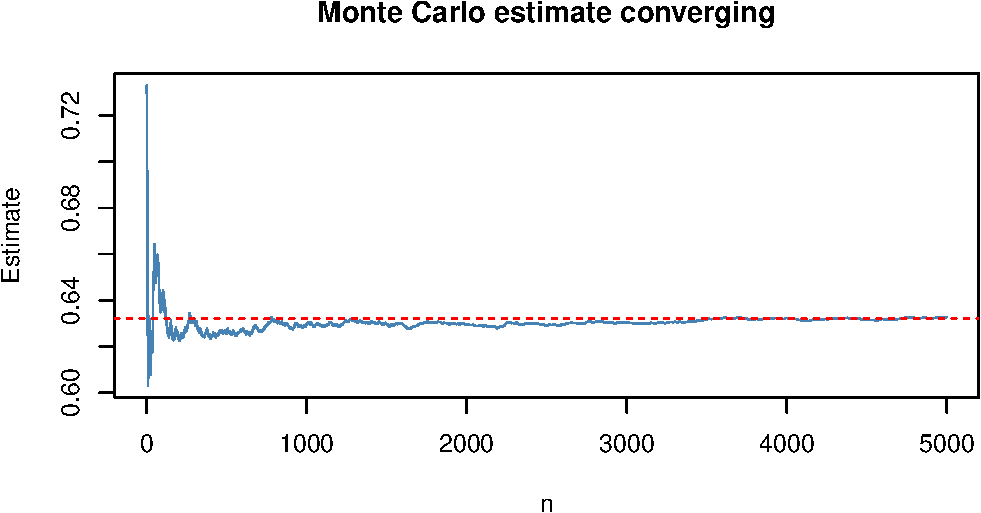
\includegraphics{04-03_Monte_Carlo_Integration_and_Importance_Sampling_files/figure-latex/ex1-plot-1} \end{center}

\subsection{Example 2: a probability}\label{example-2-a-probability}

Estimate \(P(U_1 + U_2 > 1.5)\) for independent
\(U_1, U_2 \sim \text{Uniform}(0,1)\). Elementary geometry gives the
true value \(0.125\).

\begin{Shaded}
\begin{Highlighting}[]
\NormalTok{n }\OtherTok{\textless{}{-}} \DecValTok{100000}
\NormalTok{u1 }\OtherTok{\textless{}{-}} \FunctionTok{runif}\NormalTok{(n)}
\NormalTok{u2 }\OtherTok{\textless{}{-}} \FunctionTok{runif}\NormalTok{(n)}

\NormalTok{hit }\OtherTok{\textless{}{-}}\NormalTok{ (u1 }\SpecialCharTok{+}\NormalTok{ u2) }\SpecialCharTok{\textgreater{}} \FloatTok{1.5}        \CommentTok{\# TRUE/FALSE for each draw}
\FunctionTok{c}\NormalTok{(}\AttributeTok{estimate =} \FunctionTok{mean}\NormalTok{(hit), }\AttributeTok{se =} \FunctionTok{sd}\NormalTok{(hit) }\SpecialCharTok{/} \FunctionTok{sqrt}\NormalTok{(n), }\AttributeTok{truth =} \FloatTok{0.125}\NormalTok{)}
\end{Highlighting}
\end{Shaded}

\begin{verbatim}
##    estimate          se       truth 
## 0.124780000 0.001045041 0.125000000
\end{verbatim}

\section{Importance Sampling}\label{importance-sampling}

\subsection{The problem}\label{the-problem}

Suppose \(\theta = P(Z > 4)\) with \(Z \sim N(0,1)\). The event is very
rare, with probability about \(3 \times 10^{-5}\). With 10,000 draws,
plain Monte Carlo usually sees \textbf{no hits at all} and returns
exactly 0.

For a small probability \(\theta\), the relative error of plain Monte
Carlo is

\[
\frac{\text{SE}}{\theta} \approx \frac{1}{\sqrt{n\theta}},
\]

so you need \(n \gg 1/\theta\) draws.

\subsection{The idea}\label{the-idea-1}

Sample from a different density \(p\) that visits the important region
often. Then correct each draw with a \textbf{weight}:

\[
\hat\theta_{IS} = \frac{1}{n}\sum_{i=1}^n g(Y_i)\,w(Y_i),
\qquad w(y)=\frac{f(y)}{p(y)}, \qquad Y_i \sim p
\]

This is still unbiased, because
\(E_p[g(Y)\,f(Y)/p(Y)] = \int g f\,dy = \theta\). The only requirement
is that \(p(y) > 0\) wherever \(g(y)f(y) \neq 0\).

\subsection{\texorpdfstring{How to choose
\(p\)}{How to choose p}}\label{how-to-choose-p}

The variance is smallest when \(p \propto |g|\,f\). You can't sample
from that exactly, because it needs the answer you are looking for. So
the rule of thumb is to \textbf{pick \(p\) shaped like \(|g|f\)}. For a
tail probability, that means shifting the density toward the tail.

\subsection{Method}\label{method-1}

\begin{enumerate}
\def\labelenumi{\arabic{enumi}.}
\tightlist
\item
  Choose a proposal \(p\) that puts more mass on the important region,
  with tails at least as heavy as \(f\)'s.
\item
  Draw \(Y_1,\dots,Y_n\) from \(p\).
\item
  Compute the weights \(w_i = f(Y_i)/p(Y_i)\).
\item
  Compute the values \(g(Y_i)\,w_i\).
\item
  The estimate is their mean, and the SE is their standard deviation
  divided by \(\sqrt n\).
\end{enumerate}

\subsection{Example 3: a rare event with importance
sampling}\label{example-3-a-rare-event-with-importance-sampling}

For \(P(Z>4)\), use the proposal \(N(4,1)\), which is centred at the
threshold.

\begin{Shaded}
\begin{Highlighting}[]
\NormalTok{n }\OtherTok{\textless{}{-}} \DecValTok{10000}
\NormalTok{a }\OtherTok{\textless{}{-}} \DecValTok{4}

\CommentTok{\# Plain Monte Carlo}
\NormalTok{x }\OtherTok{\textless{}{-}} \FunctionTok{rnorm}\NormalTok{(n)}
\NormalTok{g\_naive }\OtherTok{\textless{}{-}} \FunctionTok{as.numeric}\NormalTok{(x }\SpecialCharTok{\textgreater{}}\NormalTok{ a)}

\CommentTok{\# Importance sampling}
\NormalTok{y }\OtherTok{\textless{}{-}} \FunctionTok{rnorm}\NormalTok{(n, }\AttributeTok{mean =}\NormalTok{ a)                 }\CommentTok{\# draw from p = N(4, 1)}
\NormalTok{w }\OtherTok{\textless{}{-}} \FunctionTok{dnorm}\NormalTok{(y) }\SpecialCharTok{/} \FunctionTok{dnorm}\NormalTok{(y, }\AttributeTok{mean =}\NormalTok{ a)      }\CommentTok{\# w = f / p}
\NormalTok{g\_is }\OtherTok{\textless{}{-}}\NormalTok{ (y }\SpecialCharTok{\textgreater{}}\NormalTok{ a) }\SpecialCharTok{*}\NormalTok{ w}

\FunctionTok{data.frame}\NormalTok{(}
  \AttributeTok{method   =} \FunctionTok{c}\NormalTok{(}\StringTok{"Plain MC"}\NormalTok{, }\StringTok{"Importance"}\NormalTok{),}
  \AttributeTok{estimate =} \FunctionTok{c}\NormalTok{(}\FunctionTok{mean}\NormalTok{(g\_naive), }\FunctionTok{mean}\NormalTok{(g\_is)),}
  \AttributeTok{se       =} \FunctionTok{c}\NormalTok{(}\FunctionTok{sd}\NormalTok{(g\_naive) }\SpecialCharTok{/} \FunctionTok{sqrt}\NormalTok{(n), }\FunctionTok{sd}\NormalTok{(g\_is) }\SpecialCharTok{/} \FunctionTok{sqrt}\NormalTok{(n)),}
  \AttributeTok{truth    =} \DecValTok{1} \SpecialCharTok{{-}} \FunctionTok{pnorm}\NormalTok{(a)}
\NormalTok{)}
\end{Highlighting}
\end{Shaded}

\begin{verbatim}
##       method     estimate           se        truth
## 1   Plain MC 1.000000e-04 1.000000e-04 3.167124e-05
## 2 Importance 3.187168e-05 6.772927e-07 3.167124e-05
\end{verbatim}

Plain Monte Carlo gives 0 with SE 0, which looks precise but is useless.
Importance sampling lands close to the truth with a tiny standard error,
using the same \(n\).

\begin{figure}

{\centering 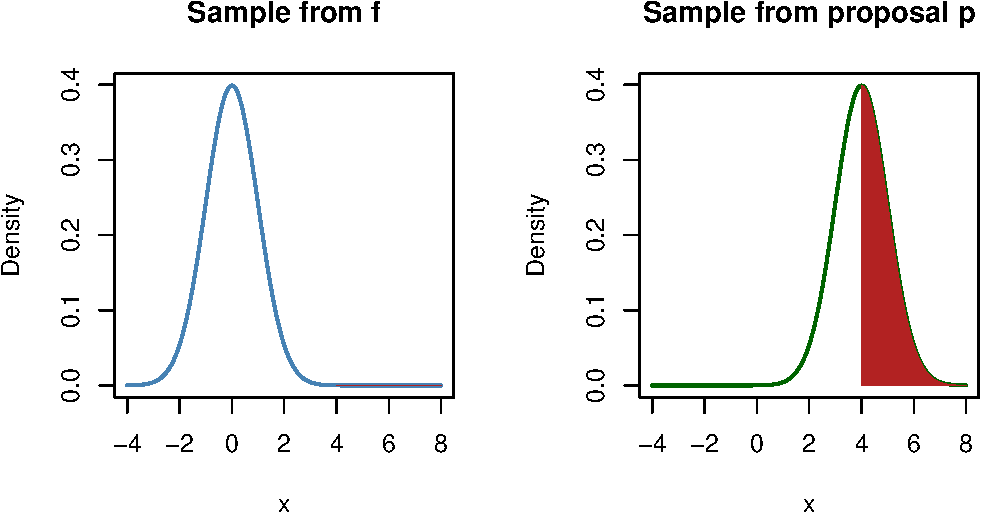
\includegraphics{04-03_Monte_Carlo_Integration_and_Importance_Sampling_files/figure-latex/ex3-plot-1} 

}

\caption{Left: f = N(0,1) rarely reaches the shaded tail. Right: the proposal N(4,1) reaches it half the time.}\label{fig:ex3-plot}
\end{figure}

\subsection{Check the weights}\label{check-the-weights}

If a few weights are huge and the rest are tiny, the proposal is a bad
match. A quick check is the \textbf{effective sample size}:

\[
n_{\text{eff}} = \frac{(\sum_i w_i)^2}{\sum_i w_i^2}
\]

If \(n_{\text{eff}}\) is much smaller than \(n\), be suspicious of the
estimate.

\begin{Shaded}
\begin{Highlighting}[]
\NormalTok{w\_all }\OtherTok{\textless{}{-}}\NormalTok{ w }\SpecialCharTok{*}\NormalTok{ (y }\SpecialCharTok{\textgreater{}}\NormalTok{ a)                    }\CommentTok{\# weights on the draws that matter}
\FunctionTok{c}\NormalTok{(}\AttributeTok{n =}\NormalTok{ n, }\AttributeTok{n\_eff =} \FunctionTok{sum}\NormalTok{(w\_all)}\SpecialCharTok{\^{}}\DecValTok{2} \SpecialCharTok{/} \FunctionTok{sum}\NormalTok{(w\_all}\SpecialCharTok{\^{}}\DecValTok{2}\NormalTok{))}
\end{Highlighting}
\end{Shaded}

\begin{verbatim}
##         n     n_eff 
## 10000.000  1813.094
\end{verbatim}

\section{Self-Normalized Importance
Sampling}\label{self-normalized-importance-sampling}

Sometimes \(f\) is known only up to a constant: \(f(x) = \tilde f(x)/c\)
with \(c\) unknown. This is typical for Bayesian posteriors. The
constant cancels if you divide by the sum of the weights:

\[
\hat\theta_{SNIS} = \frac{\sum_i g(Y_i)\,\tilde w_i}{\sum_i \tilde w_i},
\qquad \tilde w_i = \frac{\tilde f(Y_i)}{p(Y_i)}
\]

It is slightly biased for finite \(n\), but consistent.

\subsection{Example 4: unknown normalizing
constant}\label{example-4-unknown-normalizing-constant}

Take the unnormalized target \(\tilde f(x)=e^{-x^2/2}\) and estimate
\(E[X^2]\). The true value is \(1\), because the target is \(N(0,1)\).
Use the proposal \(N(0, 2^2)\).

\begin{Shaded}
\begin{Highlighting}[]
\NormalTok{n }\OtherTok{\textless{}{-}} \DecValTok{50000}
\NormalTok{y }\OtherTok{\textless{}{-}} \FunctionTok{rnorm}\NormalTok{(n, }\DecValTok{0}\NormalTok{, }\DecValTok{2}\NormalTok{)                       }\CommentTok{\# draws from p}
\NormalTok{w }\OtherTok{\textless{}{-}} \FunctionTok{exp}\NormalTok{(}\SpecialCharTok{{-}}\NormalTok{y}\SpecialCharTok{\^{}}\DecValTok{2} \SpecialCharTok{/} \DecValTok{2}\NormalTok{) }\SpecialCharTok{/} \FunctionTok{dnorm}\NormalTok{(y, }\DecValTok{0}\NormalTok{, }\DecValTok{2}\NormalTok{)       }\CommentTok{\# unnormalized weights}

\FunctionTok{sum}\NormalTok{(y}\SpecialCharTok{\^{}}\DecValTok{2} \SpecialCharTok{*}\NormalTok{ w) }\SpecialCharTok{/} \FunctionTok{sum}\NormalTok{(w)                     }\CommentTok{\# SNIS estimate (truth = 1)}
\end{Highlighting}
\end{Shaded}

\begin{verbatim}
## [1] 1.000764
\end{verbatim}

We never used the constant \(\sqrt{2\pi}\).

\section{Summary}\label{summary}

{\def\LTcaptype{none} % do not increment counter
\begin{longtable}[]{@{}
  >{\raggedright\arraybackslash}p{(\linewidth - 4\tabcolsep) * \real{0.3333}}
  >{\raggedright\arraybackslash}p{(\linewidth - 4\tabcolsep) * \real{0.3333}}
  >{\raggedright\arraybackslash}p{(\linewidth - 4\tabcolsep) * \real{0.3333}}@{}}
\toprule\noalign{}
\begin{minipage}[b]{\linewidth}\raggedright
\end{minipage} & \begin{minipage}[b]{\linewidth}\raggedright
Monte Carlo
\end{minipage} & \begin{minipage}[b]{\linewidth}\raggedright
Importance sampling
\end{minipage} \\
\midrule\noalign{}
\endhead
\bottomrule\noalign{}
\endlastfoot
Draw from & \(f\) & \(p\) (chosen by you) \\
Estimate & mean of \(g(X)\) & mean of \(g(Y)\,f(Y)/p(Y)\) \\
SE & \(s/\sqrt n\) & \(s/\sqrt n\) (of weighted values) \\
Best for & simple or high-dimensional integrals & rare events, high
variance \\
Best \(p\) & & \(\propto \lvert g\rvert f\) \\
\end{longtable}
}

\textbf{Tips}

\begin{itemize}
\tightlist
\item
  Always report a standard error.
\item
  The proposal's tails must be at least as heavy as the target's.
  Otherwise the weights can have infinite variance.
\item
  Check the weights or \(n_{\text{eff}}\).
\item
  Use self-normalized weights when the density is known only up to a
  constant.
\item
  For smooth, low-dimensional integrals, quadrature is faster. Monte
  Carlo wins as the dimension grows.
\end{itemize}

\section{Exercises}\label{exercises}

\begin{enumerate}
\def\labelenumi{\arabic{enumi}.}
\tightlist
\item
  Estimate \(\int_0^1 x^2\,dx\) by Monte Carlo and give a 95\% interval.
  The true value is \(1/3\).
\item
  Estimate \(\pi\) by simulation. Draw \((U_1,U_2)\) uniform on the unit
  square and use \(4 \times P(U_1^2+U_2^2<1)\).
\item
  Estimate \(P(Z>3)\) both ways. What is the ratio of the variances?
\item
  In Example 3, change the proposal to \(N(2,1)\) and then to
  \(N(6,1)\). Compare the SE and \(n_{\text{eff}}\).
\item
  Use a proposal with a lighter tail than the target (target \(t_3\),
  proposal \(N(0,1)\)) to estimate \(E[X^2]\). Look at the weights.
\end{enumerate}

\end{document}
